\documentclass[aspectratio=169]{beamer}
\usetheme{metropolis}

%\usepackage{beamerthemesplit}
%\beamertemplatenavigationsymbolsempty
\usepackage{amsmath}
\usepackage{amsthm}
\usepackage{amssymb}
\usepackage{latexsym}
\usepackage{graphicx}
\usepackage{fancybox}
\usepackage{dsfont}
\usepackage{multirow} 
\usepackage{multicol}
\usepackage{booktabs} 
\usepackage{dcolumn}
\usepackage{soul}
\usepackage[cache=false]{minted}
\usepackage{MnSymbol}
\usepackage{stmaryrd}


\DeclareMathOperator*{\argmax}{arg\,max}
\DeclareMathOperator*{\argmin}{arg\,min}

\newcommand{\X}{\mathtt{X}}
\newcommand{\Y}{\mathtt{Y}}

%\newcommand{\R}{\mathbb{R}}
%\newcommand{\E}{\mathbb{E}}
%\newcommand{\V}{\mathbb{V}}
\newcommand{\p}{\mathbb{P}}
\newcommand*\df{\mathop{}\!\mathrm{d}}
\newcommand{\del}{\partial}


% imports
\usepackage{xargs}
\usepackage{xpatch}
\usepackage{etoolbox}
\usepackage{pdflscape}
\usepackage{booktabs}
\usepackage{threeparttable}
\usepackage[skip=0.2\baselineskip]{caption}

% command for inputting raw latex
\makeatletter
\newcommand\primitiveinput[1]{\@@input #1 }
\makeatother

% common table command
\newcommandx{\tablecontent}[4]{
    \begin{threeparttable}[!ht]
        \centering
        \caption{#3}
        \vspace{-1em}
        \footnotesize
        \begin{tabular}{#1}
            \primitiveinput{../tables/#2.tex}
        \end{tabular}
        \vspace{-0.2em}
        \begin{tablenotes}[flushleft]
            #4
        \end{tablenotes}
    \end{threeparttable}
}




% \usepackage{slashbox}
\title{Lecture 3: Generalized Method of Moments}
\author{Chris Conlon }
\institute{NYU Stern }


\newcommand{\norm}[1]{\left\lVert#1\right\rVert}
\newcommand{\R}{\mathbb{R}}
\newcommand{\E}{\mathbb{E}}
\newcommand{\V}{\mathbb{V}}
\newcommand{\ol}{\overline}
%\newcommand{\ul}{\underline}
\newcommand{\pp}{{\prime \prime}}
\newcommand{\ppp}{{\prime \prime \prime}}
\newcommand{\policy}{\gamma}


\newcommand{\fp}{\frame[plain]}

\date{\today}

\begin{document}
\maketitle

\begin{frame}{GMM: Intro}
In the most basic setup we begin with some data $w_i$ where $i=1,\ldots,N$. Our data $w_i$ might contain all kinds of things such as dependent variables $y_i$, regressors $x_i$ and excluded instruments $z_i$. The main idea is that our economic model provides the following restriction on our data:
\begin{eqnarray*}
E[g(w_i, \theta_0) ] =0
\end{eqnarray*}
The idea is that at the true parameter value $\theta_0\in \mathbb{R}^k$ our moment conditions $g(w_i,\theta)$ are on average equal to zero. What does ``on average'' mean?  In theory, we are making an asymptotic statement about what happens as $N \rightarrow \infty$. This is what we mean when we write $E[\cdot]$.
 \end{frame}

\begin{frame}{GMM: Sample Moments}
In practice, it is helpful to consider the sample analogue, which we abbreviate with the shorthand $g_N(\theta) \in \mathbb{R}^q$, where $g_N(\theta)$ is a $q$-dimensional vector of moment conditions.
\begin{eqnarray*}
E[g(w_i, \theta )] \approx \frac{1}{N} \sum_{i=1}^N g(w_i, \theta)  \equiv g_N(\theta)
\end{eqnarray*}
\end{frame}

\begin{frame}{Other Definitions}
\begin{itemize}
\item We define the Jacobian: $D(\theta) \equiv E[\frac{\partial g(w_i,\theta)}{\partial \theta}]$, which is a $q \times k$ matrix.
\item  Evaluated at the optimum, $\frac{1}{\sqrt{N}} \sum_{i=1}^N g(w_i,\theta_0) \overset{d}{\to} N(0,S)$ where $S = E[g(w_i,\theta_0) g(w_i,\theta_0)']$ is a $q \times q$ matrix.\footnote{Technical conditions to establish this are written down later.} 
\item In other words, the moment conditions which are $0$ in expectation at $\theta_0$ are normally distributed with some covariance $S$
\item Later, we will refer to a weighting matrix $W_N$ which is a $q \times q$ positive semi-definite matrix. It tells us how much to penalize the violations of one moment condition relative to another (in quadratic distance).
\end{itemize}
\end{frame}

\begin{frame}{Examples}
It is easy to see some very simple examples:
\begin{description} 
\item[OLS] Here $y_i = x_i \beta + \epsilon_i$. Exogeneity implies that $E[x_i' \epsilon_i]=0$. We can write this in terms of just observables and parameters as $E[x_i' (y_i - x_i \beta)]=0$ so that $g(y_i,x_i, \beta) = x_i' (y_i - x_i \beta)$.
\item[IV]  Again $y_i = x_i \beta + \epsilon_i$. Now, endogeneity implies that $E[x_i' \epsilon_i]\neq0$. However there are some instruments $z_i$ which may be partly contained in $x_i$ and partly excluded from $y_i$, so that $E[z_i' \epsilon_i]=0$. $E[z_i' (y_i - x_i \beta)]=0$ so that $g(y_i,x_i,z_i, \beta) = z_i' (y_i - x_i \beta)$.
\end{description}
\end{frame}

\begin{frame}{Examples (continued)}
\textbf{Maximum Likelihood}\\
 $g(w_i,\theta) =  \frac{\partial \log f(w_i,\theta)}{\partial \theta}$ where $f(w_i,\theta)$ is the density function so that $\log f(w_i,\theta)$ is the contribution of observation $i$ to the log-likelihood. Here we set the expected (average) derivative of the log-likelihood (score) function to zero.
\end{frame}


\begin{frame}{Examples (continued)}
\textbf{Euler Equations}\\
Assume we have a CRRA utility function $u(c) = \frac{c^{1-\gamma} -1}{1-\gamma}$ and an agent who maximizes the expected discounted value of their stream of consumption. This leads to an Euler Equation:
\begin{eqnarray*}
E \left[\beta \left( \frac{c_{t+1}}{c_t} \right)^{-\gamma} R_{t+1} -1 | \Omega_t \right] =0
\end{eqnarray*}
where $\Omega_t$ is the ``Information Set'' (sigma algebra) of everything known to the agent up until time $t$ (include full histories). We can write a moment restriction of the form for any measurable $z_t \in \Omega_t$.
\begin{eqnarray*}
E \left[z_t \left(\beta  \left( \frac{c_{t+1}}{c_t} \right)^{-\gamma} R_{t+1} -1\right) \right] =0
\end{eqnarray*}
In the original work by Hansen (1982) on GMM, this $g(c_t,c_{t+1},R_{t+1},\beta,\gamma)$ was used to estimate $(\beta,\gamma)$.
\end{frame}

\begin{frame}{GMM Estimator}
Here is the GMM estimator:
\begin{eqnarray*}
\hat{\theta} = \arg \min_{\theta}  Q_N(\theta) \quad Q_N(\theta)=g_N(\theta)' W_N  g_N(\theta)
\end{eqnarray*}

\end{frame}


\begin{frame}{Technical Conditions}
\textit{These are a set of sufficient conditions to establish consistency and asymptotic normality of the GMM estimator. These conditions are stronger than necessary, but they establish the requisite LLN and CLT.}
\begin{enumerate}
\item $\theta \in \Theta$ is compact.
\item $W_N \overset{p}{\to} W$.
\item $g_N(\theta) \overset{p}{\to} E[g(z_i,\theta)]$ (uniformly)
\item $E[g(z_i,\theta)]$ is continous.
\item We need that $E[g(z_i,\theta_0)]=0$ and $W_N E[g(z_i,\theta)] \neq 0$ for $\theta \neq \theta_0$ (global identification condition).
\item $g_N(\theta)$ is twice continuously differentiable about $\theta_0$.
\item $\theta_0$ is not on the boundary of $\Theta$.
\item $D(\theta_0) W D(\theta_0)'$ is invertible (non-singular).
\item $g(z_i,\theta)$ has at least two moments finite and finite derivatives at all $\theta \in \Theta$.
\end{enumerate}
\end{frame}


\begin{frame}{GMM: Asymptotics}
The first five conditions give us consistency $\hat{\theta} \overset{p}{\to} \theta_0$ as $N \rightarrow \infty$. All nine conditions give us asymptotic normality.
\begin{eqnarray*}
\sqrt{N}(\hat{\theta}-\theta)  &\overset{d}{\to}& N(0,V_{\theta})\\
V_{\theta} &=& \underbrace{(D W D')^{-1}}_{\mbox{bread}} \underbrace{(D W S W' D')}_{\mbox{filling}}\underbrace{(D W D')^{-1}}_{\mbox{bread}} 
\end{eqnarray*}
It is common to refer parts of the variance as the \textit{bread} and the \textit{filling} or \textit{meat}, together this is referred to as the \textit{sandwich} estimator of the variance.
\end{frame}

\begin{frame}{GMM: Identification}

\begin{itemize}
\item The global identification condition is difficult to understand, for the linear model we can replace it with a (local) condition on Jacobian of the moment conditions. 
\item Recall the Jacobian: $D \equiv \frac{\partial g(w_i,\theta)}{\partial \theta}$, which is a $q \times k$ matrix. 
\item We call the problem \alert{under-identified} if $rank(D) < k$, \alert{just-identified} if $rank(D) = k$ and \alert{over-identified} if $rank(D) > k$.
\begin{itemize}
\item In the under-identified case, there may be many such $\hat{\theta}$ where $g(w_i,\hat{\theta}) =0$.
\item In the just-identified case, it should be possible to find a $\hat{\theta}$ where $g_N(\hat{\theta})=0$. 
\item We are primarily interested in the over-identified case where we will generally not find $\hat{\theta}$ which satisfies the moment conditions $g_N(\hat{\theta})\neq0$.
\end{itemize}
\item Instead, we search for $\hat{\theta}$ which minimizes the violations of the moment conditions. We write this as a quadratic form for some positive definite matrix $W_N$ which is $q \times q$.
\begin{eqnarray*}
\hat{\theta} = \arg \min_{\theta}  Q_N(\theta) \quad Q_N(\theta)=g_N(\theta)' W_N  g_N(\theta)
\end{eqnarray*}
\end{itemize}
\end{frame}

\begin{frame}{GMM: Linear IV}
For the linear IV problem this becomes:
\begin{eqnarray*}
g_N(\theta)' W_N  g_N(\theta) &=& \frac{1}{N^2} \cdot (\mathbf{Z}' (\mathbf{Y} - \mathbf{X} \beta))' W_N (\mathbf{Z}' (\mathbf{Y} - \mathbf{X} \beta)) \\
&=& \frac{1}{N^2}\cdot [Y'Z W_N Z' Y - 2 \beta X' Z W_N Z' Y + \beta' X' Z W_N Z' X \beta]
\end{eqnarray*}
We can ignore the $\frac{1}{N^2}$ and take the first-order condition:
\begin{eqnarray*}
2 X'Z W_N Z' Y &=& 2 X'Z W_N Z' X \beta\\
\hat{\beta}_{GMM} &=& (X'Z W_N Z' X)^{-1} X' Z W_N Z'Y
\end{eqnarray*}
\alert{Hopefully this looks familiar}
\end{frame}

\begin{frame}{GMM: OLS}
\begin{itemize}
\item Suppose that we do not have any excluded instruments so that $Z=X$ (and thus $q=k$). 
\item Also suppose that $W_N = \mathbf{I}_q$ (the identity matrix). 
\item Then we can see that:
\begin{eqnarray*}
\hat{\beta}_{GMM} &=& (X'X \mathbf{I}_q X' X)^{-1} X' X \mathbf{I}_q X'Y\\
 &=& (X'X X' X)^{-1} X' X X'Y\\
 &=& (X'X)^{-1} (X' X)^{-1} (X' X) X'Y =  (X'X)^{-1} X'Y = \hat{\beta}_{OLS}
\end{eqnarray*}

\item In other words, OLS is a special case of the GMM estimator.
\item  Also, the identification condition $D=\frac{\partial g(w_i,\theta)}{\partial \theta} =\frac{1}{N} \sum_{i=1}^N z_i' x_i = \frac{1}{N} \sum_{i=1}^N x_i' x_i$ becomes that $rank(X'X) = k$ the well-known OLS rank condition.\\
\end{itemize}
\end{frame}

\begin{frame}{2SLS Estimator}
Suppose that we do have excluded instruments so that $dim(Z) = q > dim(X) = k$ and that $W_N = (Z'Z)^{-1}$. It immediately follows that:
\begin{eqnarray*}
\hat{\beta}_{GMM} &=& (X'Z (Z'Z)^{-1} Z' X)^{-1} X' Z (Z'Z)^{-1} Z'Y = \hat{\beta}_{2SLS}
\end{eqnarray*}
If $dim(Z) = q = dim(X) = k$ then $(X'Z)$ is square (and invertible). This expression further simplifies:
\begin{eqnarray*}
(X'Z (Z'Z)^{-1} Z' X)^{-1} = (Z'X)^{-1} (Z'Z) (X'Z)^{-1}\\
\rightarrow \hat{\beta}_{GMM} = (Z'X)^{-1} (Z'Z) (X'Z)^{-1}  X' Z (Z'Z)^{-1} Z'Y = (Z'X)^{-1} Z'Y = \hat{\beta}_{IV}
\end{eqnarray*}
\end{frame}

\begin{frame}{Efficient GMM}
An important question remains how one should choose the weighting matrix $W_N$. We've already seen two options: 
\begin{enumerate}
\item The identity matrix $\mathbf{I}_q$ equally penalizes violations of all $q$ moments
\item  the TSLS weighting matrix $(Z'Z)^{-1}$ which can be thought about as the inverse of the covariance of the instruments. 
\end{enumerate}
We are interested in \alert{efficient GMM} which is the GMM estimator with the lowest variance.

\end{frame}

\begin{frame}{Efficient GMM}
 In order to find the $W_N$ which minimizes the variance of $\hat{\theta}_{GMM}$ we recall the asymptotic variance of the GMM estimator:
\begin{eqnarray*}
V_{\theta} =(D W D')^{-1} (D W S W' D') (D W D')^{-1}
\end{eqnarray*}
It turns out that the best choice of $W_N = S^{-1}$ (which sets $filling = bread$). This is easy to see, because $W_N$ is positive semi-definite.
\begin{eqnarray*}
(D S^{-1} D')^{-1} (D S^{-1} S S^{-1'} D') (D S^{-1} D')^{-1} = (D S^{-1} D')^{-1} (D S^{-1} D') (D S^{-1} D')^{-1} = (D S^{-1} D')^{-1}
\end{eqnarray*}
\end{frame}

\begin{frame}{Efficient GMM: Discussion}
This gives us some insight into what we are looking for from moment conditions. 

\begin{itemize}
\item We want $S$ to be small (we want the sampling variation/noise of our moments to be as small as possible). 
\item We also want $D$ (the Jacobian of the moments) to be large. 
\begin{itemize}
\item This means that small violations in moment conditions lead to large changes in the objective function. 
\item In practical terms, the problem is well identified when the objective function is steep around $\theta_0$.
\item When the problem becomes flat, it becomes hard to distinguish one $\theta$ in favor of another.
\end{itemize}
\item The problem is that $S = E[g(w_i,\theta_0) g(w_i,\theta_0)']$ is not something that we readily observe from our data. In fact, the asymptotic covariance evaluated at $\theta_0$ is \alert{infeasible}.
\end{itemize}
\end{frame}

\begin{frame}{Efficient GMM: Feasible Weight Matrix}
The best we can hope for is to use some sample analogue $W_N=\hat{S}^{-1}$ in its place. One way to compute that is the covariance of the moments estimated at some $\hat{\theta}$ for an initial guess of $W$:
\begin{eqnarray*}
\hat{W} = \hat{S}^{-1} = \left(\frac{1}{N} \sum_{i=1}^N (g(w_i,\hat{\theta}) - g_N(\hat{\theta}))  \, (g(w_i,\hat{\theta}) - g_N(\hat{\theta}))'\right)^{-1}
\end{eqnarray*}
Because $E[g(w_i,\theta_0)]=0$ at $\theta_0$ there is a tendency to use $\left(\frac{1}{N} \sum_{i=1}^N g(w_i,\hat{\theta}) \, g(w_i,\hat{\theta} )'\right)^{-1}$ (without de-meaning the moments). In theory this would work fine, but in practice \alert{it is nearly always a bad idea}.\\
\end{frame}

\begin{frame}{Efficient GMM: Review}

\noindent The overall procedure works as follows:
\begin{enumerate}
\item Pick some initial weighting matrix $W_0$: often $\mathbf{I}_q$ or $(Z'Z)^{-1}$.
\item Solve $\hat{\theta} = \arg \min_{\theta} g_N(\theta)' W_0  g_N(\theta)$.
\item Update $\hat{W} = \left(\frac{1}{N} \sum_{i=1}^N (g(w_i,\hat{\theta}) - g_N(\hat{\theta}))  \, (g(w_i,\hat{\theta}) - g_N(\hat{\theta}))'\right)^{-1}$
\item Solve $\hat{\theta}_{GMM} = \arg \min_{\theta}\, g_N(\theta)' \, \hat{W} \, g_N(\theta)$.
\item Compute $D(\hat{\theta}_{GMM})$ and $S(\hat{\theta}_{GMM})$ and compute standard errors.
\end{enumerate}
\end{frame}

\begin{frame}{Estimating the Variance Matrix}
For the linear IV estimator when $i$ is independent then $g(w_i,\theta) = z_i \epsilon_i$ and $E[z_i \epsilon_i]=0$
\begin{eqnarray*}
\hat{S}=\frac{1}{N} \sum_{i=1}^N z_i z_i' \epsilon_i^2
\end{eqnarray*}
\begin{itemize}
\item When there is homoskedastic variance $E[\epsilon_i^2 | z_i] = \sigma^2$ and the covariance of the moments becomes $\frac{\sigma^2}{N} \sum_{i=1}^N z_i z_i'$.
\item Because scaling weighting matrix by a constant has no effect on the maximum this is equivalent to the 2SLS weight matrix: $\sum_{i=1}^N z_i z_i'$ or $Z'Z$
\begin{itemize}
\item  2SLS is only the efficient estimator under \alert{homoskedasticity}.
\item  Likewise, if all regressors are exogenous then $X=Z$ and we are left with the GMM formula coincides with the covariance for heteroskedasticity robust standard errors.
\item Similarly, when appropriate we can consider extensions such as \alert{clustered standard errors} which are robust to weaker forms of independence.
\end{itemize}
\end{itemize}
\end{frame}

\begin{frame}{Estimating the Variance Matrix}
 As a practical matter, we should always use the \alert{sandwich} form when calculating the GMM standard errors, rather than the simpler \alert{bread} version which is only correct at $\theta_0$ under asymptotic optimality conditions.
\end{frame}

\section*{\normalsize  Common Questions/Extensions}

\begin{frame}{Semiparametric Efficiency}
In a famous paper, Chamberlain (1987) showed that GMM obtained the semi-parametric efficiency bound asymptotically. That means as our sample gets large and without making additional parametric assumptions (such as placing distributions on error terms) the efficient GMM provides the most efficient estimator.
\end{frame}

\begin{frame}{My first stage estimates look ok, but my second stage estimates look like garbage}
This means there is a problem with your weighting matrix. 
\begin{itemize}
\item Make sure you are subtracting off the average $g_N(\theta)$ when computing the covariance. 
\item Another problem appears is when you take the inverse. There is a statistic known as the \textit{condition number} which measures the ratio of the minimum and maximum eigenvalue of a matrix.
\begin{itemize}
\item When these eigenvalues are close together then small errors in $A+\epsilon$ lead to small errors in $(A+\epsilon)^{-1}$.
\item Software sometimes reports either the condition number, or its inverse.
\item In an ideal world this would be $\approx 1$. 
\item If the condition number is $10^{\pm 13}$ it approaches the numerical precision of your computer. 
\item Then even tiny (sampling) errors can lead to nearly infinite weighting matrices.
\end{itemize}
\end{itemize}
\end{frame}

\begin{frame}{What causes these problems?}
\begin{itemize}
\item Usually this happens if the gradient of $Q_n(\theta)$ is not close to zero in a particular dimension 
\item or the average Jacobian $D(\theta)=\frac{1}{N} \sum_{i=1}^N \frac{\partial g(w_i,\theta)}{\partial \theta}$ is not close to zero in some dimension.
\end{itemize}
You are not an optimum of $Q_n(\theta)$!
\end{frame}


\begin{frame}{My point estimates look okay, but my standard errors look crazy}
\begin{itemize}
\item You have probably dropped a $\frac{1}{N}$ or $\frac{1}{\sqrt{N}}$ somewhere.
\item  You can ignore the $N$'s when obtaining point estimates because scaling $Q_n(\theta)$ or $W_n$ does not affect the location of $\hat{\theta}$, but you need to be more careful in computing $V_{\theta}$.
\end{itemize}
\end{frame}

\begin{frame}{If 2 step GMM is good, is 3-step GMM better?}
\begin{itemize}
\item Asymptotically the answer is no
\item Even with a sub-optimal choice of weighting matrix, your first stage  $\hat{\theta} \overset{p}{\to}\theta_0$ as $N \rightarrow \infty$.
\item  This means that in the limit, you always recover the efficient choice of $\hat{W}$.
\item  In finite sample, anything can happen, but numerous studies have found little to no improvement from considering a $K$-step GMM estimator.
\end{itemize}
\end{frame}

\begin{frame}{What about Infinite-step GMM?}
 There isn't such a thing. But there is the \alert{Continuously Updating GMM} estimator of Hansen Heaton and Yaron (1996). In this case we let \\
\begin{align*}
W(\theta)&=\left(\frac{1}{N} \sum_{i=1}^N (g(w_i,\theta) - g_N(\theta)) (g(w_i,\theta)-g_N(\theta))' \right) \\
Q_n(\theta)^{CUE} &= g_N(\theta)' \left(\frac{1}{N} \sum_{i=1}^N (g(w_i,\theta) - g_N(\theta)) (g(w_i,\theta)-g_N(\theta))' \right) g_N(\theta)
\end{align*}
\begin{itemize}
\item Because the weighting matrix now changes with $\theta$, even for linear models this becomes very difficult to estimate. 
\item The original GMM problem was a quadratic optimization problem. The CUE problem is no longer a convex optimization problem. Quasi-Newton approaches are no longer guaranteed to work.
\end{itemize}
\end{frame}

\begin{frame}{Advanced Asymptotics}
\small
CUE has some additional advantages over GMM. We see this by examining the GMM FOC. 
\begin{eqnarray*}
\hat{D}(\theta) W_n \hat{g}_N(\hat{\theta}) =0
\end{eqnarray*}
If we take an Edgeworth expansion we can see how the  \alert{asymptotic bias} term looks:
\begin{eqnarray*}
\frac{1}{N^2}\sum_{i=1}^N E[g(w_i,\theta) W_n g(w_i,\theta)]
\end{eqnarray*}
As long as the variance is finite we can see that this bias disappears as $N \rightarrow \infty$. However it also tends to grow linearly with $q$ the number of moment restrictions. This is often referred to as the \textit{too many moments} or \textit{many instruments} problem.

The challenge is that in general when we estimate $\hat{g}(\hat{\theta})$ and $\hat{D}(\hat{\theta})$ we construct them so that they are mechanically correlated with one another. It turns out the CUE estimator fixes this in exactly the right way. How is beyond the scope of this note (and course). If you are really interested you should look at Newey and Smith (2004).

\end{frame}

\section{Testing}

\begin{frame}{Testing with MLE}
Before we discuss testing under GMM, let's look at testing under MLE.
\begin{itemize}
\item Helpful to define the \alert{likelihood ratio}
\begin{align*}
LR \equiv -2 \cdot \frac{\mathcal{L}(\theta_1 | x)}{\mathcal{L}(\theta_2 | x)} = -2 \cdot \left[ \ell(\theta_1 | x) - \ell(\theta_2 | x) \right]
\end{align*}
\item Consider $\dim(\theta_1) = q_1$ and $\dim(\theta_2) = q_2$ \alert{number of restrictions}
\item Often we let $\theta_2$ be the \alert{unrestricted} and $\theta_1$ be the \alert{restricted} model.
\item Define the degrees of \alert{degrees of freedom} $N - \dim(\theta)$.
\item The $LR$ statistic is distributed:
\begin{align*}
 \Lambda \sim \chi^2_{q_1-q_2}
\end{align*}
\item If we know $\theta_1$ and $\theta_2$ and we fix significance level $\alpha =0.05$ then \alert{Neyman-Pearson Lemma} says this is \alert{uniformly post powerful test}.
\end{itemize}
\end{frame}

\begin{frame}{Testing with MLE}
We can consider the more advanced possiblity:
\begin{align*}
L R=-2 \ln \left[\frac{\sup _{\theta \in \Theta_{0}} \mathcal{L}(\theta)}{\sup _{\theta \in \Theta} \mathcal{L}(\theta)}\right]
\end{align*}
\begin{itemize}
\item $\Theta_0$ is a restricted version of the larger set $\Theta$.
\item We can also consider \alert{non nested tests} by looking at differences in \alert{degrees of freedom}
\begin{itemize}
\item This is mostly beyond what we will do in this course.
\end{itemize}
\end{itemize}
\end{frame}

\begin{frame}{GMM: J-test}
The equivalent test in GMM is the \alert{J-test}
\begin{align*}
Q_N(\theta)&=g_N(\theta)' W_N  g_N(\theta) \\
N \cdot Q_N(\theta) &\rightarrow^D \chi^2_{n-k}
\end{align*}
This is an $LR$-type test statistic.
\end{frame}


\begin{frame}{Inverting LR tests}
A useful technique is that we can always \alert{invert} a test statistic in order to construct confidence intervals.
\begin{itemize}
\item Form an unrestricted estimate $\widehat{\theta}_{MLE}$ or $\widehat{\theta}_{GMM}$
\item Compute $\ell(\widehat{\theta})$.
\item Find all of the $\theta$ such that  $CI=\{\theta: \ell(\widehat{\theta}) -  \ell(\theta) < c \}$.
\item If we do $GMM$ we can use the $J$-stat instead.
\end{itemize}
How to choose $c$ the \alert{critical value}.
\begin{itemize}
\item Compute the number of degrees of freedom / additional restrictions
\item Choose a significance level $\alpha$ (ie: $\alpha=0.05$).
\end{itemize}
\end{frame}


\begin{frame}{Confidence Intervals and Wald Tests}
The multivariate Wald Test is:
\begin{align*}
H_{0}: R \theta=r \quad &
H_{1}: R \theta \neq r\\
\left(R \hat{\theta}_{n}-r\right)^{\prime}\left[R\left(\hat{V}_{n} / n\right) R^{\prime}\right]^{-1}\left(R \hat{\theta}_{n}-r\right) \quad &\rightarrow \quad \chi_{Q}^{2}
\end{align*}
\begin{itemize}
\item $R$ is a matrix of $q$ linear restrictions on $K$ parameters.
\item $\hat{V}_n$ is the covariance matrix for $\widehat{\theta}$.
\end{itemize}
You've been constructing CI's this way already
\begin{align*}
\widehat{\beta} \pm 1.96 SE(\widehat{\beta})
\end{align*}
\end{frame}

\begin{frame}{LM or Score Test}
There is a third test known as the \alert{Score Test} or \alert{LM Test}
\begin{align*}
S(\theta)&=\frac{\partial \ell(\theta | x)}{\partial \theta} \\
I(\theta)&=-E\left[\frac{\partial^{2}}{\partial \theta^{2}} \ell(X ; \theta) | \theta\right]
\end{align*}
\begin{itemize}
\item Compute the \alert{score of log likelihood}
\item Compute the \alert{Fisher Information}.
\item The test statistic\
\begin{align*}
S^{T}\left(\hat{\theta}_{0}\right) I^{-1}\left(\hat{\theta}_{0}\right) S\left(\hat{\theta}_{0}\right) \sim \chi_{q}^{2}
\end{align*}
Where $q$ is number of restrictions and $\theta_0$ is the true value.
\end{itemize}
\end{frame}

\begin{frame}{The Trinity of Testing}
\begin{center}
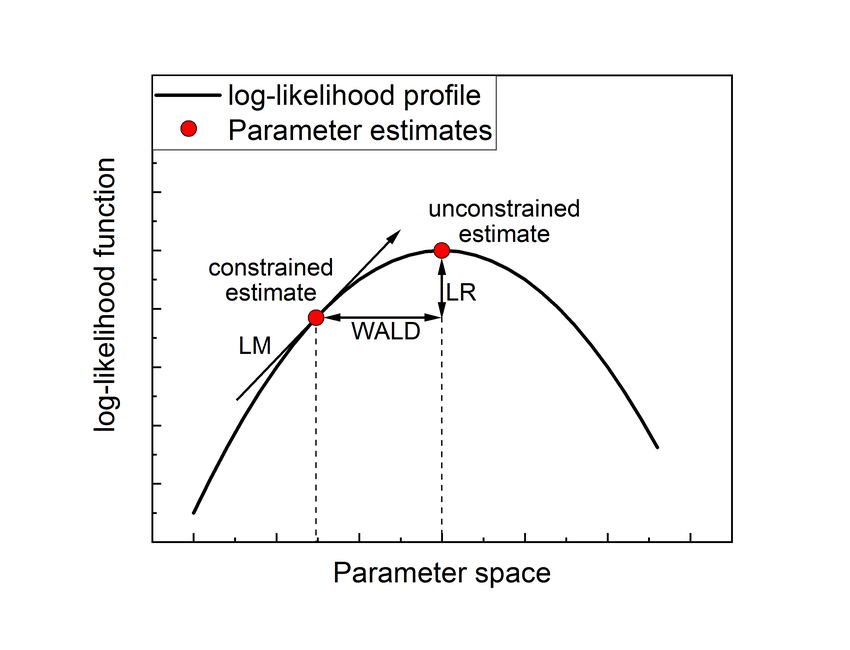
\includegraphics[height=\textheight]{./resources/lmlrwald.png}
\end{center}
\end{frame}

\begin{frame}{What to do in practice?}
\begin{itemize}
\item By reporting asymptotic standard errors you are implicitly using \alert{Wald} type statisitics.
\item If you are comparing models, you should probably try an \alert{LR} type statistic if you can.
\begin{itemize}
\item It used to be people didn't do this because $LR$ required maximizing the objective function more than once.
\item But computers today are pretty good...
\end{itemize}
\item For most extremum estimators (MLE, GMM, GEL, etc.) there are all three kinds of test-statistics
\begin{itemize}
\item ... and around the true $\theta_0$ as $N\rightarrow \infty$ they should coincide.
\item but in finite sample... anything can happen!
\end{itemize}

\end{itemize}

\end{frame}
\section*{Thanks!}

\end{document}